\newcommand\ddfrac[2]{\frac{\displaystyle #1}{\displaystyle #2}}

\chapter{Testing Parallelisation Efficiency}

\textbf{N.B: My code has changed significantly since Milestone 2, it has been committed to the MS3 directory of the provided SVN repository.}

\section{Test Framework}
To offset the tedious work of running the numerous tests outlined by the initial testing plan, the Python script developed for the basic testing carried out in Chapter 1 was extended to automate the process for both strong and weak testing. As such, the procedure for reproducing these results consists of only eleven commands, these can be found in Appendix \ref{app:framework}. 
This was accomplished by programmatically populating a \lstinline{slurm} template (found in Appendix \ref{app:template}) and submitting tasks using \lstinline{sbatch}. The script was also used to collate and summarise the output of the tests, producing both the results charts found below, and CSV reports of the findings. Single jobs can also be run by populating the template and running \lstinline{sbatch template.sh}.

\section{Deviations from Initial Test Plan}
Due to unforeseen limitations imposed by the available hardware on the \lstinline{goliath} and \lstinline{getafix} clusters where the tests were performed, both strong and weak scaling plans needed to be revised. Specifically, the fact that each node of the coursework partition contains only 64 cores proved a limiting factor. This was expected, but what was not expected was that the allocation of each thread to OpenMP would require the exclusive utilisation of a whole core.

\subsection{Strong Scaling}
% Table, Count, Technology Used
The strong scaling test plan was the most severely affected by the limitations described above. Previous plans to have configurations containing up to 32 threads were scrapped, and more configuration options were added due to the relative ease of assigning them programmaticaly. This primarily consisted of ensuring that each task/node configuration was tested using all compatible thread configurations. The final set of configurations can be found in Appendix \ref{app:actual-strong}. All tests were conducted on a problem size of 10,000 characters.

\subsection{Weak Scaling}
Due to a fundamental misunderstanding about how tests for weak scaling were to be performed, the test input sizes needed to be seriously curtailed as tests of 10,000 or 100,000 characters (per processing unit) would not be feasible due to the time limits imposed by the course. Test results for an input length of 1 character were discarded as they consisted entirely of noise. The final input length options are included in the table below. Each test of each configuration was conducted twenty times for each input size (problem size/processing unit). 
% Table, Count, Size Choice Justification

\begin{table}[H]
\centering
\begin{tabular}{|l|}
\hline
\multicolumn{1}{|c|}{\textbf{\begin{tabular}[c]{@{}c@{}}Input Size\\ (per processing unit)\end{tabular}}} \\ \hline
10 \\ \hline
100 \\ \hline
1000 \\ \hline
\end{tabular}
\caption{Actual Weak Scaling Input Magnitudes}
\label{tab:real-weak}
\end{table}


\section{Test Results}
\subsection{Strong Scaling}

Strong scaling tests were conducted on both the \lstinline{goliath} and \lstinline{getafix} clusters . A summary of mean results across the 20 samples collected for each configuration is included in Appendix \ref{app:strong-res}. Figure \ref{fig:strong-results} below shows the aggregated performance of the program on a fixed problem size of 10,000 characters, with varying combinations of MPI processes and OpenMP threads.

\begin{figure}[H]
\centering
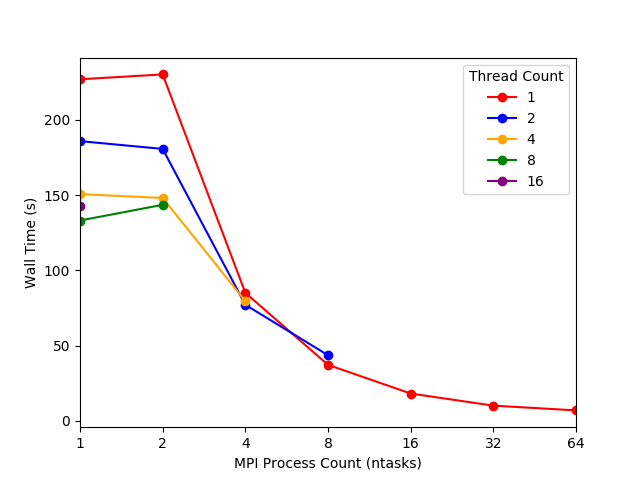
\includegraphics[width=10cm]{img/strong.png}
\caption{Strong Scaling Results}
\label{fig:strong-results}
\end{figure}

\subsubsection{Multi-threading Performance}
As can be seen in Figure \ref{fig:strong-results}, the addition of OpenMP threads has a distinct impact on overall run-time, particularly for configurations consisting of few MPI processes. However, the effect of additional threads has a diminishing rate of return, and can even be detrimental. This can be seen in the one-task, 16-thread configuration that has demonstrably worse performance than the one-task, eight-thread configuration even when averaged over 20 samples. The positive impact also (at $\geq$ 8 threads) diminishes quite rapidly; for example, the first additional thread reduces compute time by ~18\%, but it takes an additional two processes to achieve an additional performance impact of the same magnitude. More threads may have a significantly more beneficial impact on larger problem sizes, where the diagonal length of sub-sections far outstrips the number of threads available.

\subsubsection{Multi-processing Performance}
The addition of processes also had a clearly positive effect, far more impactful than that of threads. There is one notable exception, at the configuration involving two-task, one thread, which performed worse than with one-task. This makes sense in the context of the segmentation heuristic responsible for allocating work to child processes. Due to the complex nature of splitting the problem, configurations with two processes will short-circuit to using a single processor. Given the overhead of setting up a process and not using it, the difference in performance at $ntasks=2$ is to be expected. This problem is discussed in greater detail in section 3.5.3, below.

\subsection{Weak Scaling}

A summary of mean results across the 20 samples collected for each configuration of weak testing is included in Appendix \ref{app:weak-res}. Figure \ref{fig:weak-results} below plots the weak scaling results for the three different problem sizes (per unit). 

\begin{figure}[H]
\centering
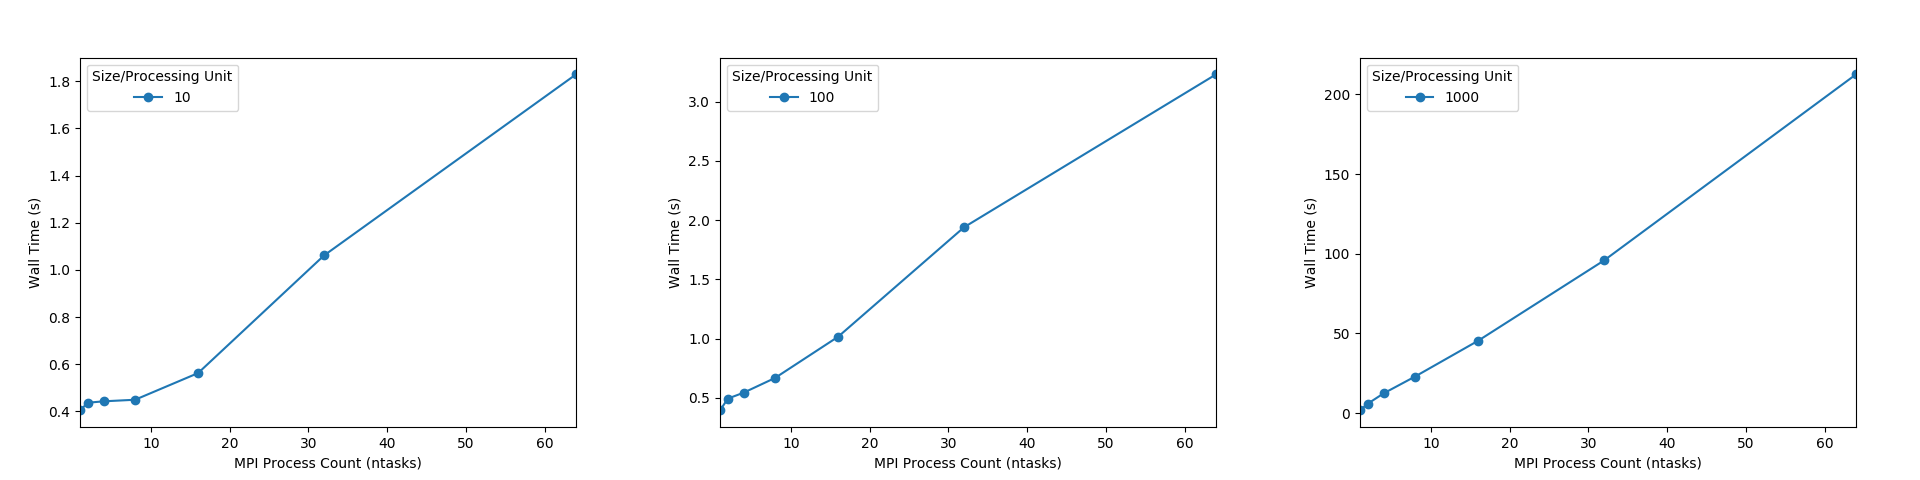
\includegraphics[width=18cm]{img/weak.png}
\caption{Weak Scaling Results}
\label{fig:weak-results}
\end{figure}

All three problem magnitudes appear to be growing extremely linearly with increased processing units and respective problem size, excepting a small amount of noise in the $n=10$ test results. This is deceptive, as we shall see in the efficiency analysis, because the absolute extent of the gradient is hidden by the axes' limits being set relative to the data points.

\section{Scaling Efficiency}
\subsection{Strong Scaling Efficiency}
Despite the strong apparent showing of the results in the previous section, examining the results in terms of "speed-up" relative to a serial solution, showed several surprising results. The following formula was used to calculate the actual speedup:
$$\frac{runtime_{serial}}{runtime_{parallel}}$$
This was compared to the theoretical maximum speedup as proposed by Amdahl \cite{Amdahl}, calculated with the following formula:
$$\frac{1}{\frac{f(N)}{p} + (1 - f(N))}$$
Where $N$ is the problem size, $p$ is the number of processing units and $f(N)$ is the proportion of the program's run-time that can be parallelised. Both threads and processes, given their requirement for a single core per unit, were treated as coequal processing units in the graph below. Due to the overwhelming proportion of time in the parallelisable section, this figure was set at 0.95 (i.e. 95\% of time was spent in parallelisable sections).

\begin{figure}[H]
\centering
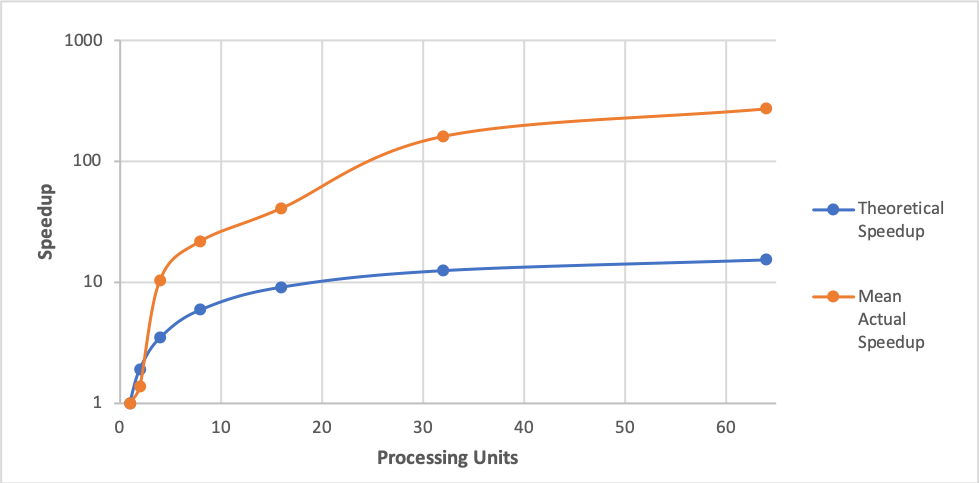
\includegraphics[width=10cm]{img/strong-scaling.png}
\caption{Strong Scaling Efficiency}
\label{fig:strong-efficiency}
\end{figure}

The first thing that stands out is that the actual speedup almost immediately overshoots the theoretical maximum by a non-trivial amount (note the logarithmic scale of the vertical axis). While this should not theoretically be possible (and had to be verified to ensure it was not a mistake) there are numerous possible explanations for this, the most likely being that the serial solution has been made artificially slow by the modification of the code to allow for the possibility of parallelisation. Other possible reasons could include environmental factors, though this is less likely due to the fact that twenty iterations were conducted and the mean taken.

\subsection{Weak Scaling Efficiency}

Weak scaling efficiency was calculated using the same formula as strong scaling, with a correction for the increasing problem size:
$$\frac{runtime_{pserial}}{runtime_{parallel} / processing\, units}$$
The theoretical maximum was calculated in accordance with the rule proposed by Gustafson \cite{Gustafson}:
$$p + (1 - p) \cdot T_{serial}$$
Where $T_{serial}$ is the proportion of time spent on serial (or non-parallelisable) sections of code.

\begin{figure}[H]
\centering
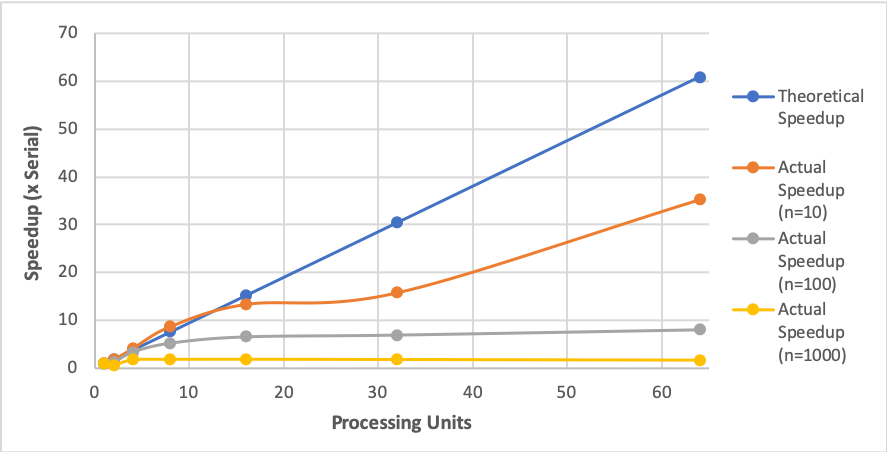
\includegraphics[width=10cm]{img/weak-scaling.png}
\caption{Weak Scaling Efficiency}
\label{fig:weak-efficiency}
\end{figure}

These figures are far more inline with expected behaviour, though below eight processing units the speedup still exceeded the theoretical maximum. Again, this could be due to noise given the small problem size, but the excessive sensitivity to the serial time is more likely to blame.

The behaviour of the tests at the $n=1000$ level was somewhat unexpected, as the larger problem size should have offset a lot of the communication and setup overhead, but on further inspection it became apparent that the communication load grows linearly with the problem size. However, this does not explain why the performance at this level is so much worse than linear. This could suggest a severe overestimation of the parallelisable proportion of the code, but such a hypothesis would not be consistent with the results of the strong scaling tests.

\section{Findings}
\subsection{Impediments}
There were numerous instances in which errors in programming or test design led to less than satisfactory outcomes during the course of development and testing of the parallel LCS solution. Several of the most impactful of these have been summarised below: 
\begin{itemize}
    \item Memory Allocation: initial phases of testing were conducted under simple conditions, and total input size never exceeded a character length of 10,000 (resulting in a table size of 100 million elements). However, on proceeding to larger input sizes, memory allocation for the table contained in the master process began to fail. In order to optimise on memory usage, the entire codebase was translated from using C++ \lstinline{std::vector} objects to using raw integer arrays to store the master and sub-section tables. This proved insufficient, as it later emerged that the master table was being constructed (duplicated) in every process, despite being unused in worker processes. Removal of this bug allowed for normal operation until significantly larger problem sizes (\textgreater 2.5 billion element master tables) where the problem re-emerged. This was solved by requesting larger memory allocations in the \lstinline{slurm} shell scripts submitted to \lstinline{sbatch}.
    \item Resource Binding: another problem encountered due to my relative naivete with respect \lstinline{slurm} and programming for clusters was not realising that, by default, OpenMP threads allocated to the job will be bound to a single core. This was overcome by passing the \lstinline{--bind-to none} flag to \lstinline{mpirun}. The incredible impact of this change on performance can be seen in Figure \ref{fig:resource-binding}, though these results were confounded by a change in cluster from \lstinline{goliath} to \lstinline{getafix}. Notice in particular the order of magnitude change in run time. This reduced run time also impacts the uniformity of the results, despite both test runs containing the same number of samples.
    \begin{figure}[H]
    \centering
    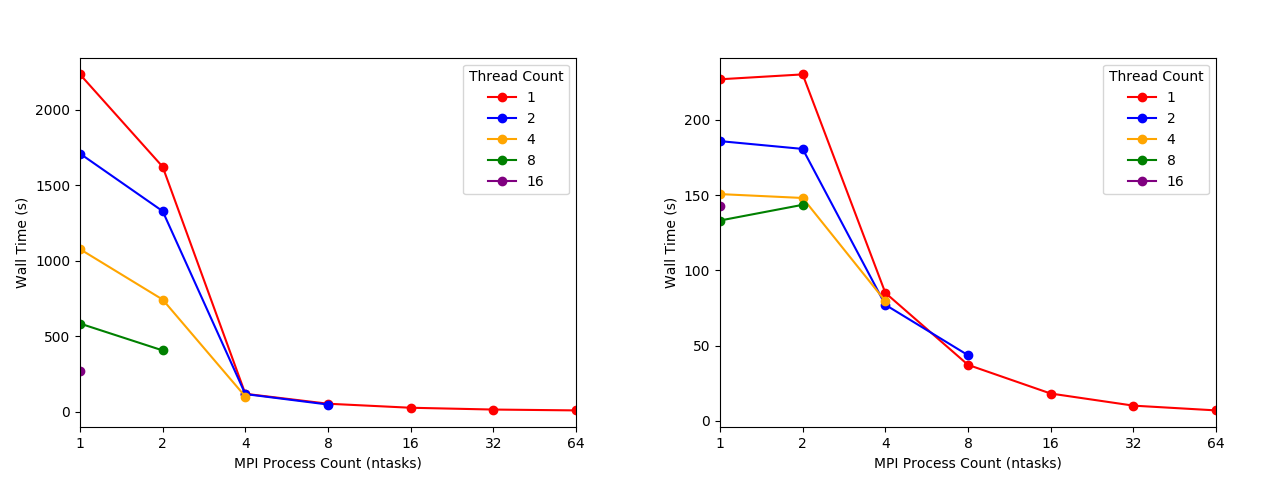
\includegraphics[width=18cm]{img/resource-binding.png}
    \caption{Pre-Resource Binding (left, goliath) and Post Resource Binding (right, getafix)}
    \label{fig:resource-binding}
    \end{figure}
    \item Level of Threading Support: my initial plans for parallelising the distribution of work to worker processes involved using OpenMP to have each send and receipt completed by a separate thread, IO-heavy work being a perfect place to implement threading. Unfortunately this implementation would have required a level of threading support (\lstinline{MPI_THREAD_MULTIPLE}) not supported on either \lstinline{goliath} or \lstinline{getafix} (both of which only support \lstinline{MPI_THREAD_SERIALIZED}); the level being set at compile-time (both clusters being compiled). This would have allowed for OpenMP multi-threading in both the master and worker classes simultaneously. Though not implemented, alternative options for parallelising this section are discussed below.
\end{itemize}

\subsection{Strengths}

The primary strength of the approach taken is that it takes full advantage of the multi-processing capabilities of the clusters on which it was tested. By utilising the diagonal calculation methodology at both the thread and process level, the program was able to achieve speed-ups in excess of the theoretical maximum. Though this is likely due to poor serial performance, it does indicate that the parallelisation has been particularly successful.

\subsection{Weaknesses \& Possible Improvements}

There are numerous areas in which the program, as written, lacks sophistication and could stand to be improved. Three of the most serious issues have been detailed below.

\subsubsection{Problem Division}
By far the greatest weakness of the parallel algorithm as it stands is the relatively naive way in which the problem space is divided into sub-problems, and the way these sub-problems are allocated to worker processes.

The diagonal calculation algorithm utilised in the program is most efficient when sub-sections are perfectly square. This enables the most threads to simultaneously calculate cells. The present heuristic divides the total problem into $n \cdot n$ subsections (where $n$ is the number of processes), without considering the dimensions of the problem. A more advanced heuristic considering these factors, and the relative importance of prioritising the size optimality of the whole problem (where each sub-section is dealt with by processes) against that of the subsections (where each cell on a diagonal may be calculated by independent threads). Dynamic detection of the number of and threads (in addition to that of processes, which is already utilised) may assist in optimising performance in this area.

\subsubsection{Allocation}
In order to simplify the process of allocating and distributing process, the program short-circuits parallel operation for any less than three processors, due to difficulties imposed by the previously mentioned segmentation heuristic. Optimally, the actual segmentation would remain unchanged, but each sub-section would be allocated to the sole worker process in order. The master process could also be utilised for more actual calculations, making use of the downtime between sending and receiving large sub-sections from worker processes.

\subsubsection{Distribution}
Due to numerous, significant, and time-consuming problems in implementing asynchronous behaviour, all MPI send and receive operations are conducted synchronously. It is strongly recommended that the sending of sub-section data to worker processes and the receipt of completed sub-sections be conducted in parallel. The nature of the algorithm would necessitate that all sub-sections on a diagonal be finished before the next begins. Hence, an \lstinline{MPI_Waitall} will be required between diagonals. There is no discernible benefit in asynchronously sending and receiving on the worker-process end, due to the linear nature of their operation.

\subsection{Further Scaling}
The range of testing configurations was severely limited by the resources allocated to the course, specifically the number of nodes available on the \lstinline{getafix} $cosc$ and \lstinline{goliath} $coursework$ partitions. Time was also a limiting factor as due to the shared nature of these resources.

In order to support truly massive input sizes, the program would need to be modified to offset limitations imposed by a lack of available hardware. 

Memory proved to be the most pressing resource constraint in the small-scale testing conducted for this report, and there is no reason to expect this would not be the case for even larger input sizes. The sheer size of the master table (already in the billions of elements for conducted tests) will eventually result in a lack of sufficient RAM to store the table. This could be offset by keeping only those values necessary for computation in memory and storing already computed values on disk. Entire sections could be saved to files and reloaded on demand. This would introduce additional IO overhead, but may be unavoidable and would certainly be offset by sufficient processing gains. This would also have the advantage of providing progress "checkpoints" that may allow for the resumption of processing in the event of interruption.

Processing power will also (eventually) hit physical limitations. It may be worth modifying the division of the problem such that the number of segments on the major anti-diagonal outnumbers the process count, such that each each segment is computable in a reasonable amount of time with the (potentially) limited resources of each node. This would introduce additional logical complexity in the distribution and receipt of segments, but may produce additional performance gains in the event of a cluster consisting of a high number of low resource nodes.